\documentclass{article}
\usepackage[utf8]{inputenc}
\usepackage[margin=0.5in,includefoot]{geometry}
\usepackage[export]{adjustbox}
\usepackage{amsmath}
\usepackage{hyperref}

% Header and Footer Setup
\usepackage{fancyhdr}
\pagestyle{fancy}
\fancyhead{}
\fancyfoot{}
\fancyfoot[R]{\thepage}
\renewcommand{\headrulewidth}{0pt}
\renewcommand{\footrulewidth}{0pt}
%
%Graphics Setup
\usepackage{graphicx}
\usepackage{float}
\usepackage{subfig}


%list setup
\usepackage{amssymb}
\renewcommand{\labelitemi}{$\blacktriangleright$}
\renewcommand{\labelitemii}{$\bullet$}
\renewcommand{\labelitemiii}{$\circ$}

%Source Code setup
\usepackage{xcolor}
\usepackage{listings}

\definecolor{mGreen}{rgb}{0,0.6,0}
\definecolor{mGray}{rgb}{0.5,0.5,0.5}
\definecolor{mPurple}{rgb}{0.58,0,0.82}
\definecolor{backgroundColour}{rgb}{0.95,0.95,0.92}

\lstdefinestyle{CStyle}{
   tabsize = 4, 
	showstringspaces = false, 
	numbers = left,
	commentstyle=\color{mGreen}, 
	keywordstyle = \color{blue},
	stringstyle = \color{red}, 
	rulecolor = \color{black}, 
	basicstyle = \small \ttfamily, 
	breaklines = true, 
	numberstyle = \tiny,
	language = Java ,
	frame = trBL , 
	firstnumber = 1
}


%


\begin{document}

\begin{titlepage}

	\begin{flushright}
	\textsc{\large November 4, 2021} \\
	\end{flushright}
	\begin{center}
	\Large{\bfseries GTU Department of Computer Engineering \\ CSE 484/654 Natural Language Processing \\ Fall 2021 - Homework 1 Report  } \\
	\end{center}
	\topskip0pt
	\vspace*{\fill}
	\begin{center}
	\Large{\bfseries Akif Kartal \\ 171044098 }
	\end{center}
	\vspace*{\fill}

\end{titlepage}

\cleardoublepage
\section{Problem Definition} 
The problem is to make experiments with vector representation of words for turkish language.

\section{Solution}
The homework was finished as expected in homework pdf file. 
\subsection{Creating corpus}
To create big turkish text, I have used a NodeJs library with javascript. Check the following picture.
\begin{figure}[H]
    \centering
	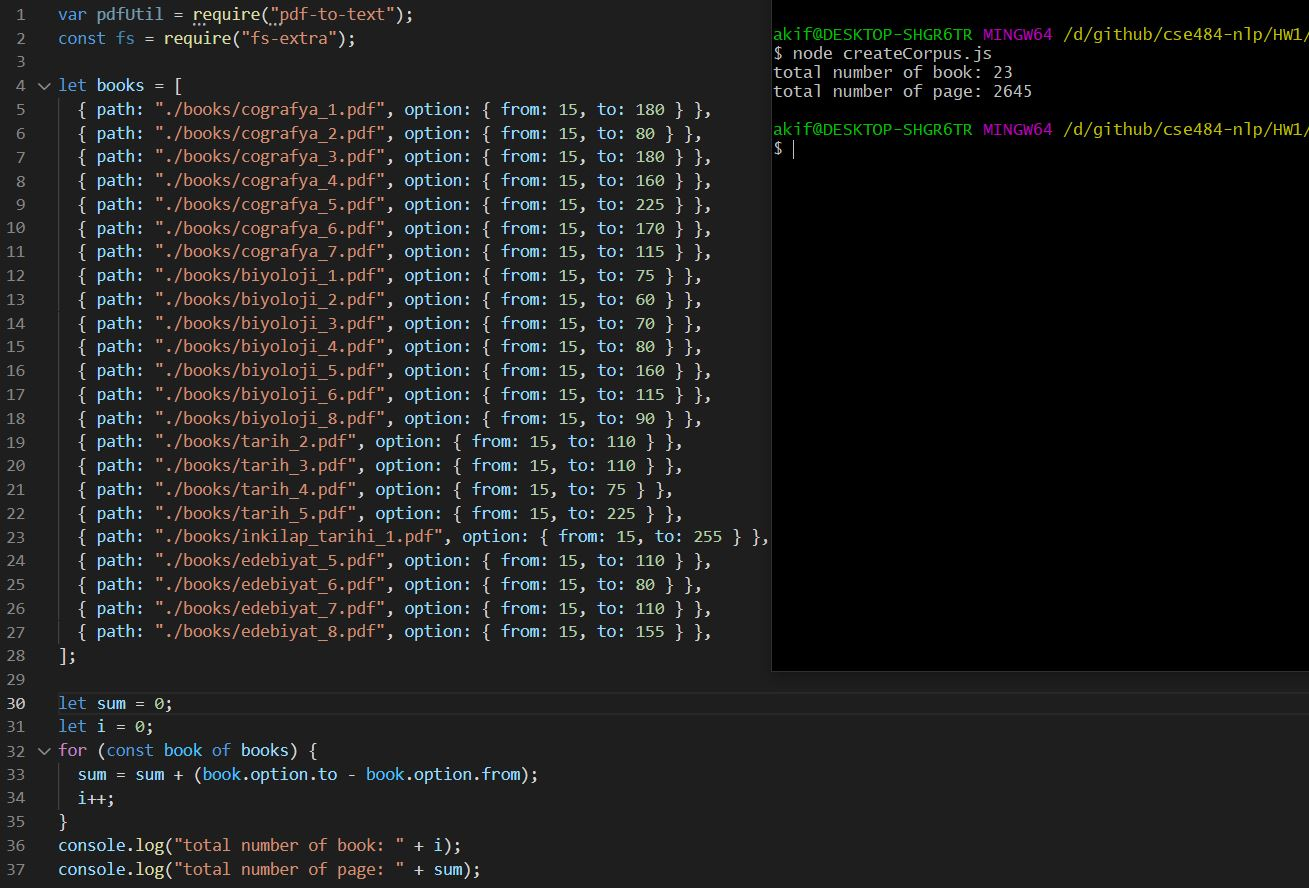
\includegraphics[width=7in, height=5in]{3.JPG}
	\caption[Optional caption]{Program to create text file(corpus)}
	\label{}
\end{figure}
You can see the books and their used page numbers from picture. I have 2645 page text with 23 book. \\
\newline
Following code piece is showing how I convert pdf to text. Note that I converted pdfs to
text by \textbf{removing all new line feeds} such as carriage return, line feed, tabs etc. Also I converted all words to \textbf{lower case} in order to make proper compare with syllable based text.
\cleardoublepage
\subsubsection{Convert pdfs to one line text file}
\begin{figure}[H]
    \centering
	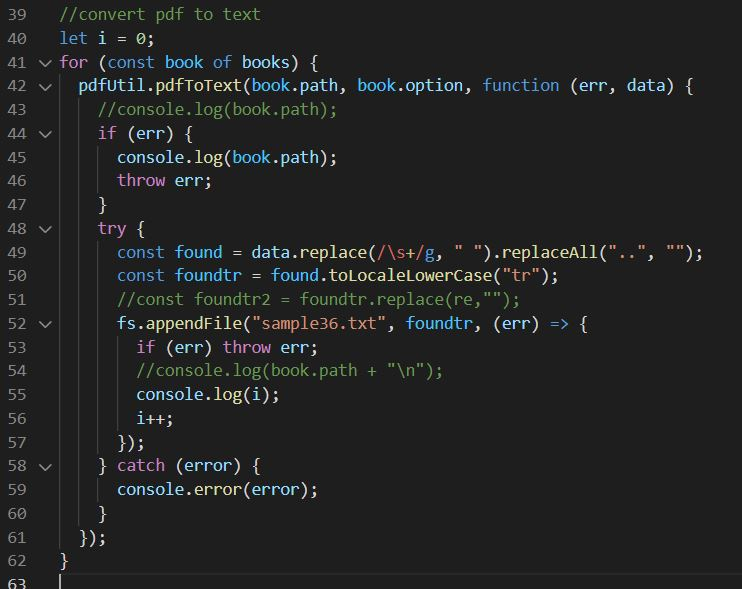
\includegraphics[width=6in, height=4in]{4.JPG}
	\caption[Optional caption]{Convert pdfs to text file}
	\label{}
\end{figure}
\begin{figure}[H]
    \centering
	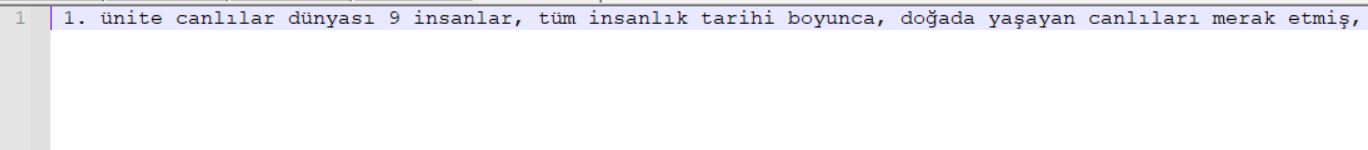
\includegraphics[width=7in, height=2in]{5.JPG}
	\caption[Optional caption]{Converted text file}
	\label{}
\end{figure}
\subsubsection{Testing created text vectors}
Following pictures contains some examples of distance and anology experiment on created text corpus with word2vec C code.
\begin{figure}[H]
    \centering
	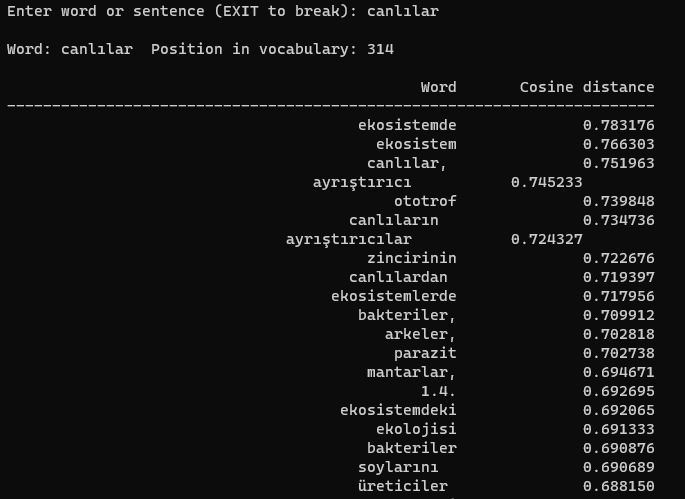
\includegraphics[width=6in, height=4in]{8.JPG}
	\caption[Optional caption]{Distance test with canlılar word}
	\label{}
\end{figure}
\begin{figure}[H]
    \centering
	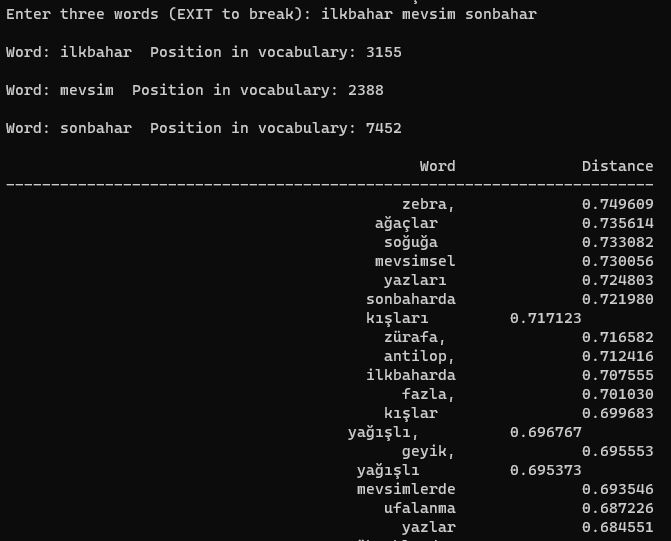
\includegraphics[width=6in, height=4in]{11.JPG}
	\caption[Optional caption]{Anology test with ilkbahar mevsim sonbahar words}
	\label{}
\end{figure}
\subsection{Dividing Turkish words into syllables}
In order to divide turkish words into syllables, I have used following open source python library. \\
\newline
\url{https://github.com/MeteHanC/turkishnlp}
\newline
\newline
\newline
Code to divide syllables is following;
\begin{figure}[H]
    \centering
	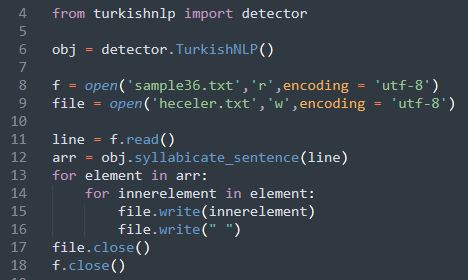
\includegraphics[width=6in, height=3in]{6.JPG}
	\caption[Optional caption]{Simple code to divide words into syllables}
	\label{}
\end{figure}
\begin{figure}[H]
    \centering
	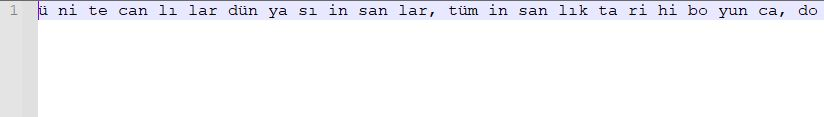
\includegraphics[width=5in, height=2in]{7.JPG}
	\caption[Optional caption]{Syllables of words after dividing}
	\label{}
\end{figure}
\subsection{Word similarity accuracy}
In order to find similarity between two vector we will use cosine similarity formula.
\begin{figure}[H]
    \centering
	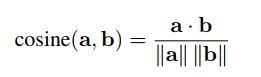
\includegraphics[width=3in, height=0.7in]{15.JPG}
	\caption[Optional caption]{cosine similarity formula}
	\label{}
\end{figure}
\begin{figure}[H]
    \centering
	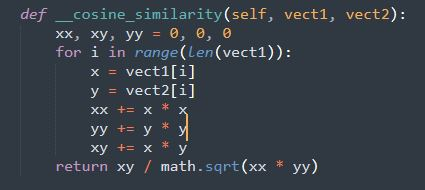
\includegraphics[width=4in, height=2in]{16.JPG}
	\caption[Optional caption]{Implementation of cosine similarity formula}
	\label{}
\end{figure} 
\subsection{Measuring the accuracy}
In order to measure accuracy of algorithm, we will use following formula.
\begin{figure}[H]
    \centering
	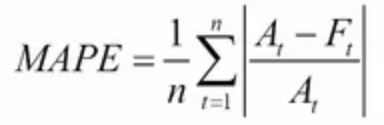
\includegraphics[width=3in, height=1in]{19.JPG}
	\caption[Optional caption]{Mean Absolute Percentage Error formula}
	\label{}
\end{figure}
As seen above,we initially calculate the absolute difference between the Actual Value(Human Score)(A) and the Experiment(cosine similarity of two word)(F) value.
\begin{figure}[H]
    \centering
	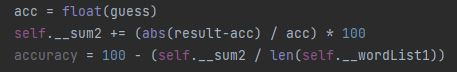
\includegraphics[width=4in, height=0.7in]{20.JPG}
	\caption[Optional caption]{Simple implementation of MAPE formula}
	\label{}
\end{figure} 
\cleardoublepage
\subsection{Syntactic distance accuracy}
Here we have 20 turkish Syntactically similar words and their human scores.
\begin{figure}[H]
    \centering
	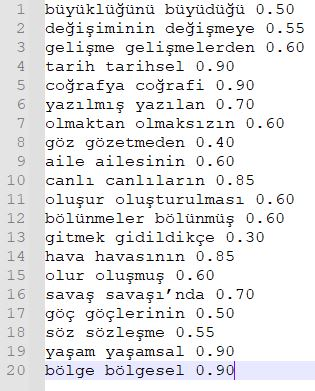
\includegraphics[width=4in, height=4in]{18.JPG}
	\caption[Optional caption]{Syntactically similar words and their human scores(0-1)}
	\label{}
\end{figure}
\cleardoublepage
\begin{figure}[H]
    \centering
	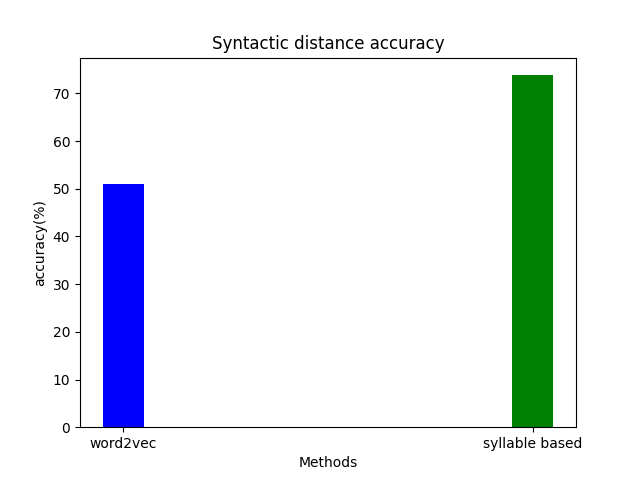
\includegraphics[width=6in, height=4in]{syn_dist.png}
	\caption[Optional caption]{Syntactic distance accuracy of algorithms with above words}
	\label{}
\end{figure}
As you can see from graph \textbf{syllable based} algorithm is much more successful with in syntactic distance accuracy. \\
\newline
\textbf{Semantic distance accuracy} \\
\newline
Here we have 15 turkish semantically  similar word and their human scores.
\begin{figure}[H]
    \centering
	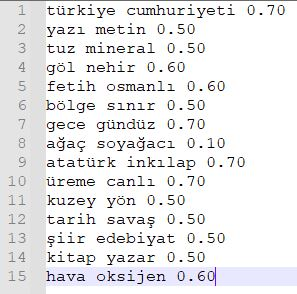
\includegraphics[width=4in, height=3in]{17.JPG}
	\caption[Optional caption]{Semantically similar word and their human scores(0-1)}
	\label{}
\end{figure}
\begin{figure}[H]
    \centering
	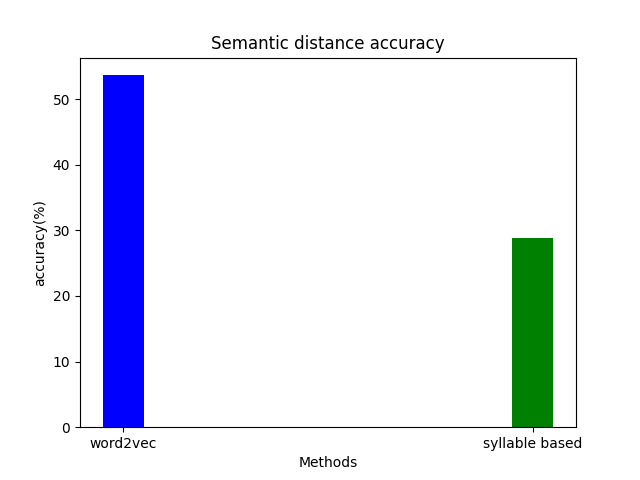
\includegraphics[width=6in, height=4in]{seman_dist.png}
	\caption[Optional caption]{Semantic distance accuracy of algorithms with above words}
	\label{}
\end{figure}
As you can see from graph \textbf{word2vect} algorithm is much more successful with in semantic distance accuracy. \\
\newline
\textbf{Full results}
\begin{figure}[H]
    \centering
	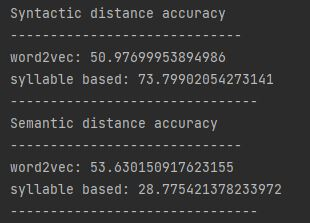
\includegraphics[width=4in, height=3in]{24.JPG}
	\caption[Optional caption]{Distance accuracy results(\%)}
	\label{}
\end{figure}
\cleardoublepage
\subsection{Word analogy accuracy}
In order to measure analogy, we will use following formulas.
\begin{figure}[H]
    \centering
	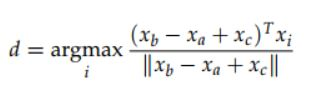
\includegraphics[width=3in, height=1in]{21.JPG}
	\caption[Optional caption]{Full formula}
	\label{}
\end{figure}
\begin{figure}[H]
    \centering
	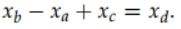
\includegraphics[width=3in, height=0.4in]{22.JPG}
	\caption[Optional caption]{With the vectors}
	\label{}
\end{figure}  



\subsubsection{Syntactic analogy accuracy}
Here we have 5 turkish syntactically similar analogy words and their human scores.
\begin{figure}[H]
    \centering
	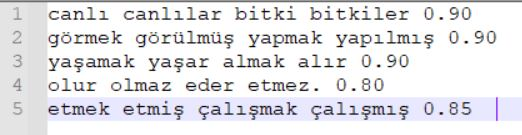
\includegraphics[width=4in, height=2in]{25.JPG}
	\caption[Optional caption]{Syntactically similar analogy words and their human scores(0-1)}
	\label{}
\end{figure}
Here, in order to calculate analogy we will use cosine similarity. \\
\newline 
For example; \\
\newline
\text{similarity(vector[bitkiler], vector[canlılar] + vector[bitki] - vector[canlı] )}
\newline
\newline
\newline
After getting similarity ratio then we will measure accuracy with human score. You can see resuts from graph.
\begin{figure}[H]
    \centering
	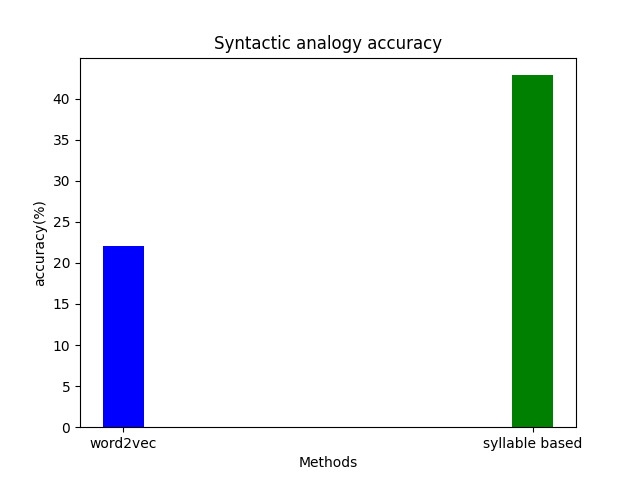
\includegraphics[width=6in, height=4in]{syn_anal.png}
	\caption[Optional caption]{Syntactic analogy accuracy of algorithms with above words}
	\label{}
\end{figure}
As you can see from graph \textbf{syllable based} algorithm is much more successful with in syntactic analogy accuracy. 
\subsubsection{Semantic analogy accuracy}
Here we have 5 turkish semantically similar analogy words and their human scores.
\begin{figure}[H]
    \centering
	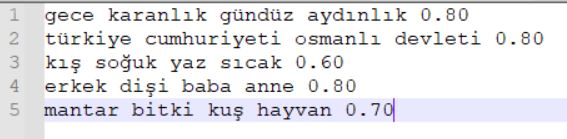
\includegraphics[width=5in, height=2.5in]{26.JPG}
	\caption[Optional caption]{Semantically similar analogy words and their human scores(0-1)}
	\label{}
\end{figure}
\begin{figure}[H]
    \centering
	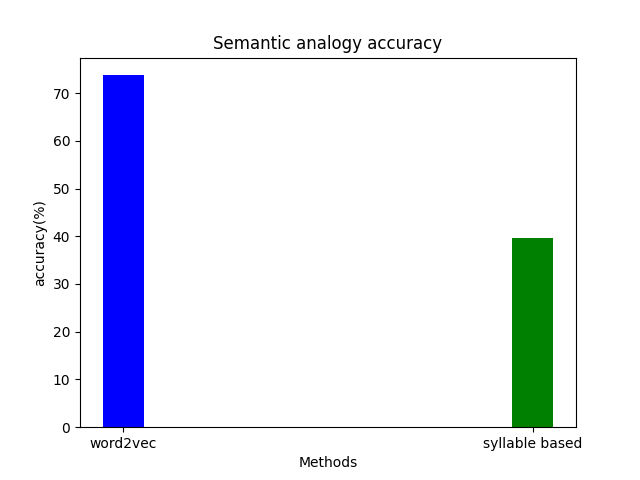
\includegraphics[width=6in, height=4in]{sem_anal.png}
	\caption[Optional caption]{Semantic analogy accuracy of algorithms with above words}
	\label{}
\end{figure}
As you can see from graph \textbf{word2vect} algorithm is  more successful with in semantic analogy accuracy. \\
\newline
\textbf{Full results}
\begin{figure}[H]
    \centering
	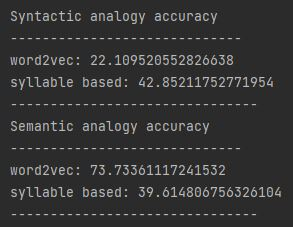
\includegraphics[width=4in, height=3in]{27.JPG}
	\caption[Optional caption]{Analogy accuracy results(\%)}
	\label{}
\end{figure}

\textbf{How to ensure my algorithm is working}
\newline
\newline
My distance and analogy algorithms works as perfect as word2vec C code. You can see results from image with same input files.
\begin{figure}[H]
    \centering
	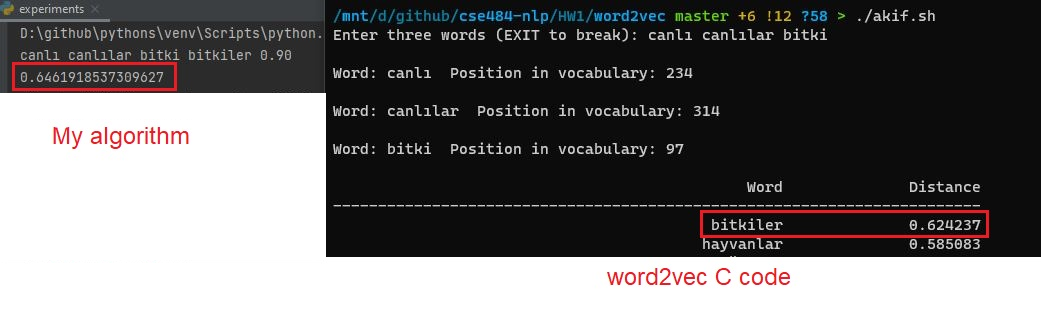
\includegraphics[width=7in, height=3in]{res.png}
	\caption[Optional caption]{Compare with word2vec C code with same input files}
	\label{}
\end{figure}

\section{References} 
\begin{itemize}
	\item cs224n-2020-lecture02-wordvecs2.pdf file from lecture notes
	\item \url{https://cs224d.stanford.edu/lecture_notes/notes2.pdf}
	\item \url{https://github.com/MeteHanC/turkishnlp}
	\item \url{https://www.npmjs.com/package/pdf-to-text}
	\item \url{http://aok.meb.gov.tr/kitap/}
	\item \url{https://github.com/tmikolov/word2vec}
	\item \url{https://www.geeksforgeeks.org/graph-plotting-in-python-set-1/}
\end{itemize}
\section{How to run}
Just install needed python libraries and run 171044098.py file. If you want, you can change test input words, but be sure word is present in vector file. 
   
\end{document}